\section{Autopilot Design}
You can answer Problem 1 in this file/section. One subsection for each part of the problem might be a good solution.

\subsection{}
The first order Nomoto model is a simple vessel model that we can use for this problem. The transfer function from rudder angle $\delta$ to heading rate $r = \dot \psi$ is given by equation (7.28) in \cite{Fossen2011} and is
\begin{equation}\begin{aligned}
\frac{r}{\delta}(s) = \frac{K}{Ts + 1}
\end{aligned}\end{equation}
This corresponds to the time-domain representation
\begin{equation}\begin{aligned}
T \ddot \psi + \dot \psi = K \delta.
\end{aligned}\end{equation}

\begin{figure}[ht]
	\centering
	\begin{subfigure}[b]{0.45\textwidth}
		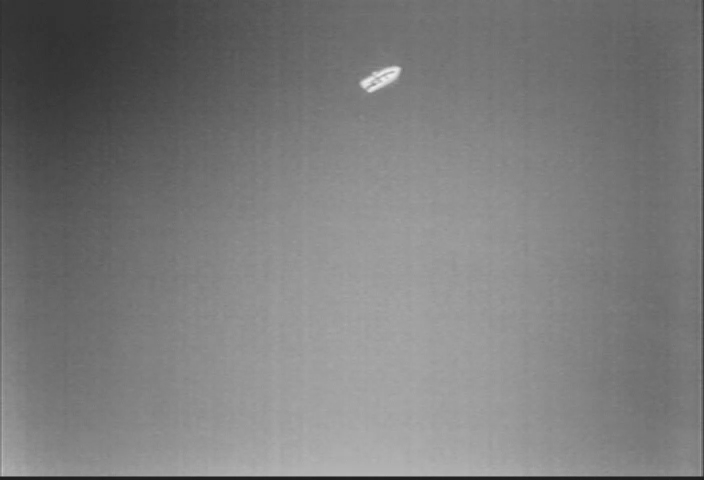
\includegraphics[width=\textwidth]{fig1}
		\caption{caption..}
		\label{fig:2a}
	\end{subfigure}
	~ %add desired spacing between images, e. g. ~, \quad, \qquad, \hfill etc.
	%(or a blank line to force the subfigure onto a new line)
	\begin{subfigure}[b]{0.45\textwidth}
		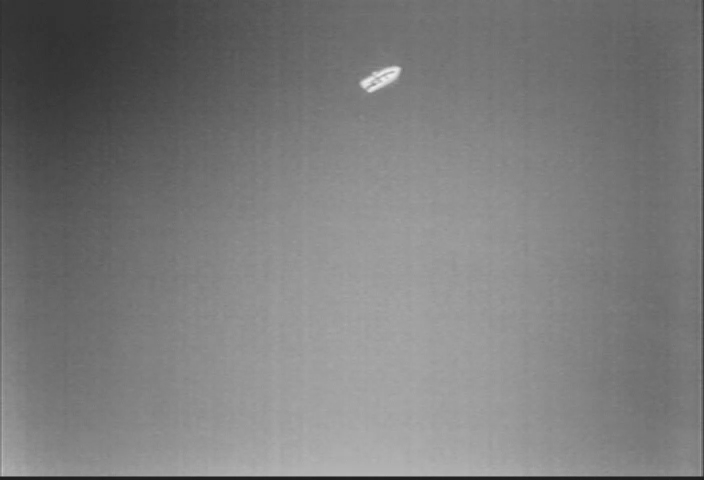
\includegraphics[width=\textwidth]{fig1}
		\caption{caption..}
		\label{fig:2b}
	\end{subfigure}
	\begin{subfigure}[b]{0.45\textwidth}
		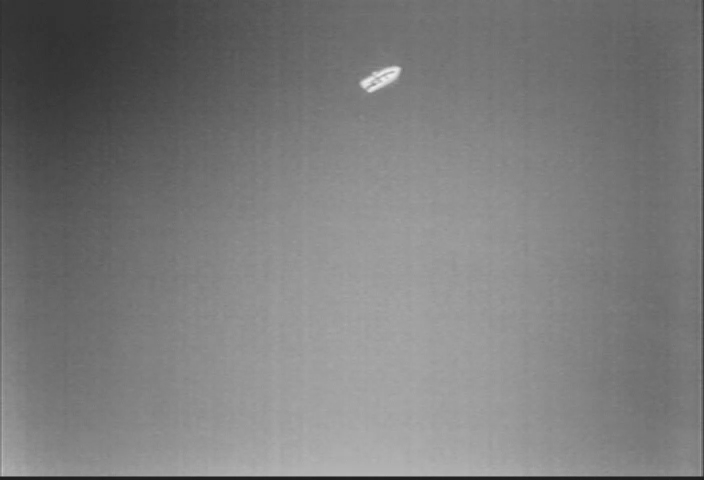
\includegraphics[width=\textwidth]{fig1}
		\caption{caption..}
		\label{fig:2c}
	\end{subfigure}
	\begin{subfigure}[b]{0.45\textwidth}
		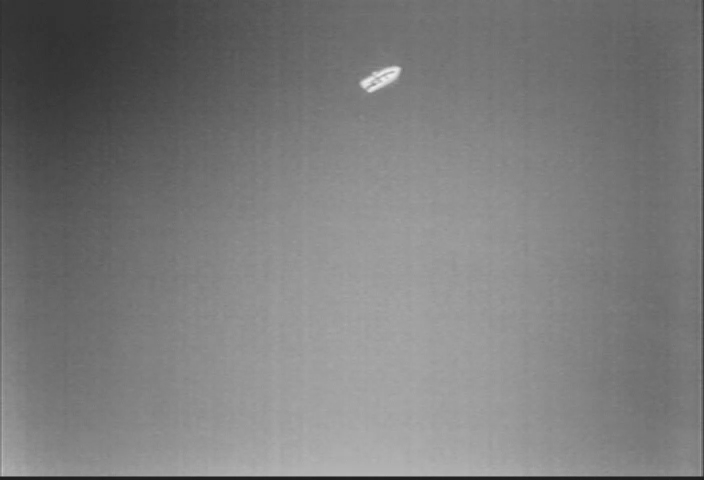
\includegraphics[width=\textwidth]{fig1}
		\caption{caption..}
		\label{fig:2d}
	\end{subfigure}
	\caption{Caption for all figures}\label{fig:2}
\end{figure}


